\documentclass{article}
\usepackage[letterpaper,margin=0.95in]{geometry}
\usepackage[T1]{fontenc}
\usepackage{graphicx,parskip,fancyhdr}
\usepackage[most]{tcolorbox}
\pagestyle{fancy}
\fancyhf{}
\lhead{CMU 16-831}\chead{Introduction to Robot Learning}\rhead{Fall 2026}
\cfoot{\thepage}
\setlength{\headheight}{14pt}
\newtcolorbox{answer}[1]{colback=white,colframe=black!60,title={#1},height=4.5cm}
% For each plot, change {example-image-a} to your image path, such as
% {figures/q3_reacher.png}. Keep the image dimensions and answer blocks unchanged.
\begin{document}
\begin{center}{\Large Assignment 4: Model-Based Reinforcement Learning}\end{center}
\textbf{Andrew ID:} vawale\par
\textbf{Collaborators (including AI tools, if applicable):} No human collaborators. Claude (Anthropic) helped with the code and the text format.\par
\textbf{Total: 15 points.} Keep the answer and plot sizes unchanged.
\section*{Problem 1: Dynamics Model Training (3.75 points)}
\begin{answer}{Which model performs best, and why?}
The model with 2 hidden layers of 250 units and 500 training steps is the best. Its MPE is 0.028 and its final training loss is 0.12. The 1x32 model with 500 steps has an MPE of 0.21. The 2x250 model with 5 steps has an MPE of 1.26, and its predictions stay almost flat. The large network has more capacity, thus it can fit the nonlinear cheetah dynamics better. But a large network also needs sufficient gradient steps, and 5 steps are not sufficient to fit the data.
\end{answer}
\begin{tcolorbox}[colback=white,colframe=black!60,title={1 hidden layer, 32 units, 500 training steps},height=9.5cm]
\centering
% Replace example-image-a with the path to your plot.
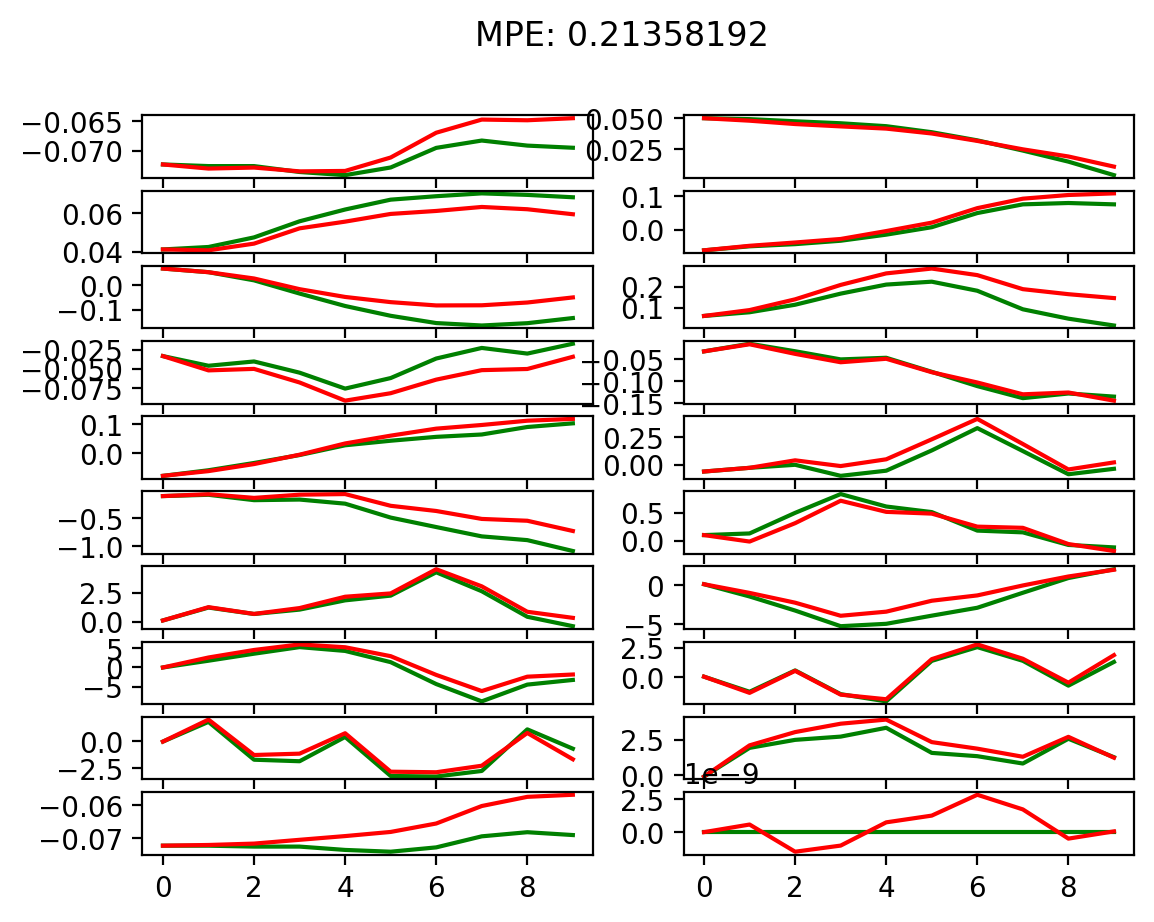
\includegraphics[width=\linewidth,height=8cm,keepaspectratio]{figures/q1_cheetah_n500_arch1x32.png}
\end{tcolorbox}
\begin{tcolorbox}[colback=white,colframe=black!60,title={2 hidden layers, 250 units, 5 training steps},height=9.5cm]
\centering
% Replace example-image-a with the path to your plot.
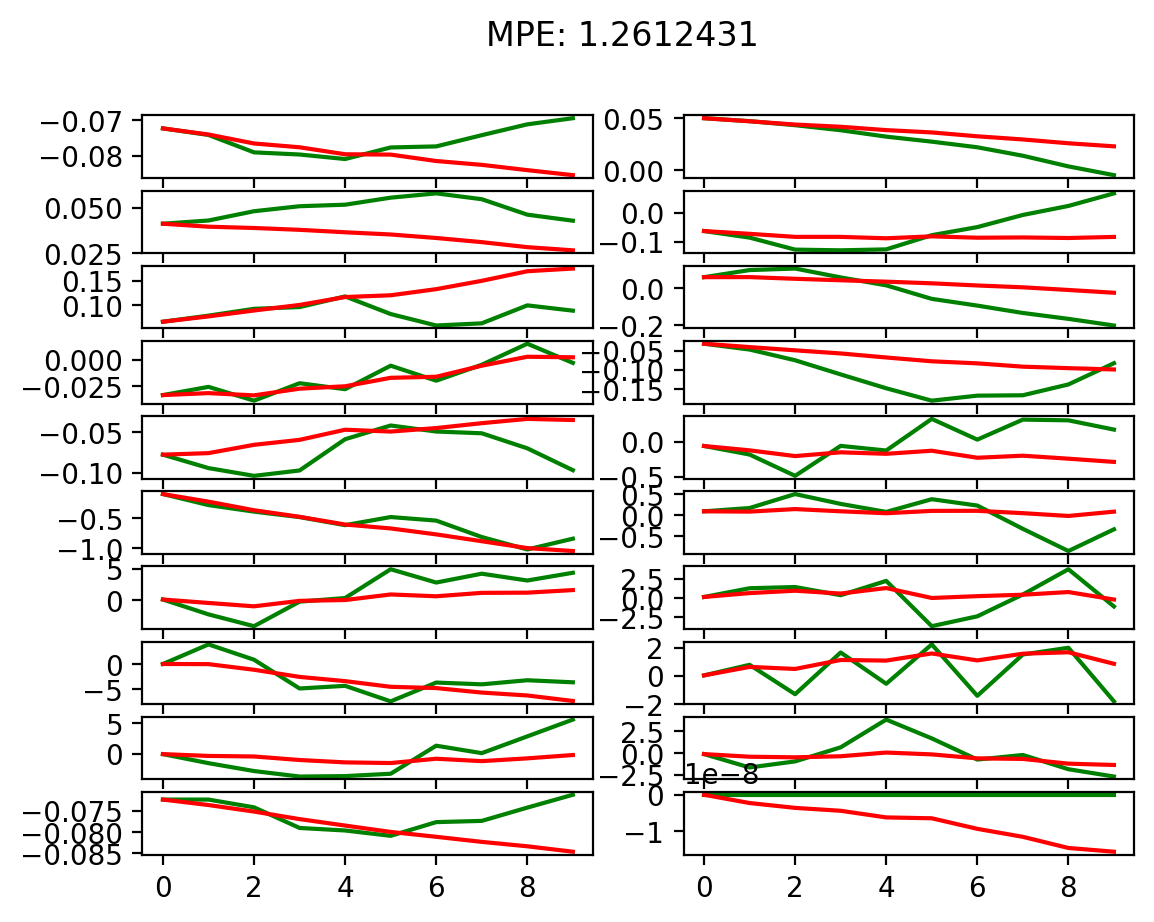
\includegraphics[width=\linewidth,height=8cm,keepaspectratio]{figures/q1_cheetah_n5_arch2x250.png}
\end{tcolorbox}
\begin{tcolorbox}[colback=white,colframe=black!60,title={2 hidden layers, 250 units, 500 training steps},height=9.5cm]
\centering
% Replace example-image-a with the path to your plot.
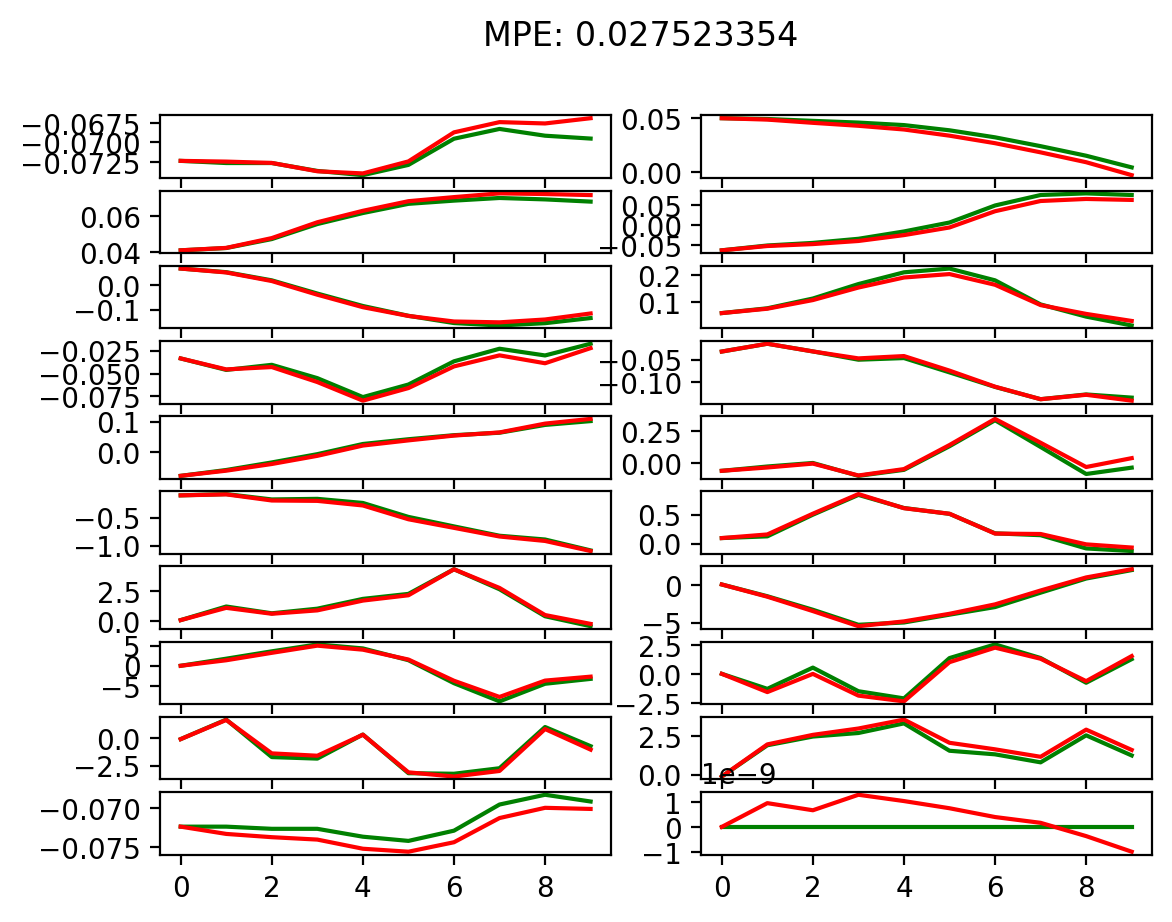
\includegraphics[width=\linewidth,height=8cm,keepaspectratio]{figures/q1_cheetah_n500_arch2x250.png}
\end{tcolorbox}
\section*{Problem 2: Action Selection (3.75 points)}
\begin{tcolorbox}[colback=white,colframe=black!60,title={Random actions versus MPC: training and evaluation returns},height=9.5cm]
\centering
% Replace example-image-a with the path to your plot.
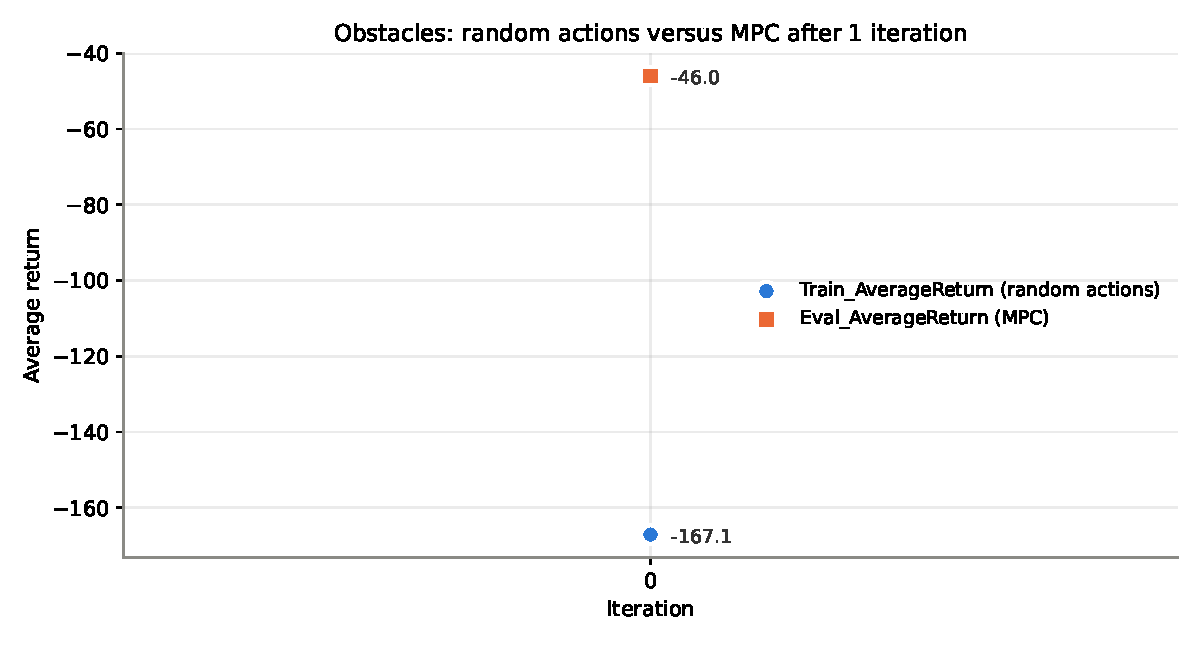
\includegraphics[width=\linewidth,height=8cm,keepaspectratio]{figures/q2_obstacles.pdf}
\end{tcolorbox}
\section*{Problem 3: Iterative Model Training (3.75 points)}
\begin{tcolorbox}[colback=white,colframe=black!60,title={Obstacles learning curve},height=9.5cm]
\centering
% Replace example-image-a with the path to your plot.
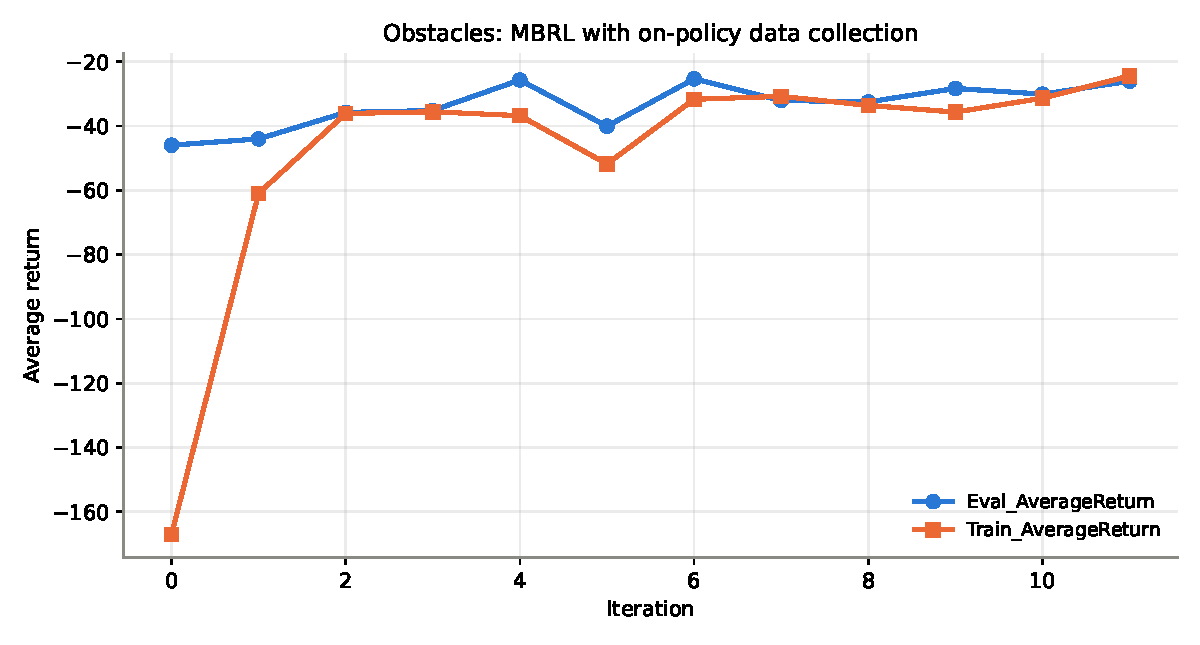
\includegraphics[width=\linewidth,height=8cm,keepaspectratio]{figures/q3_obstacles.pdf}
\end{tcolorbox}
\begin{tcolorbox}[colback=white,colframe=black!60,title={Reacher learning curve},height=9.5cm]
\centering
% Replace example-image-a with the path to your plot.
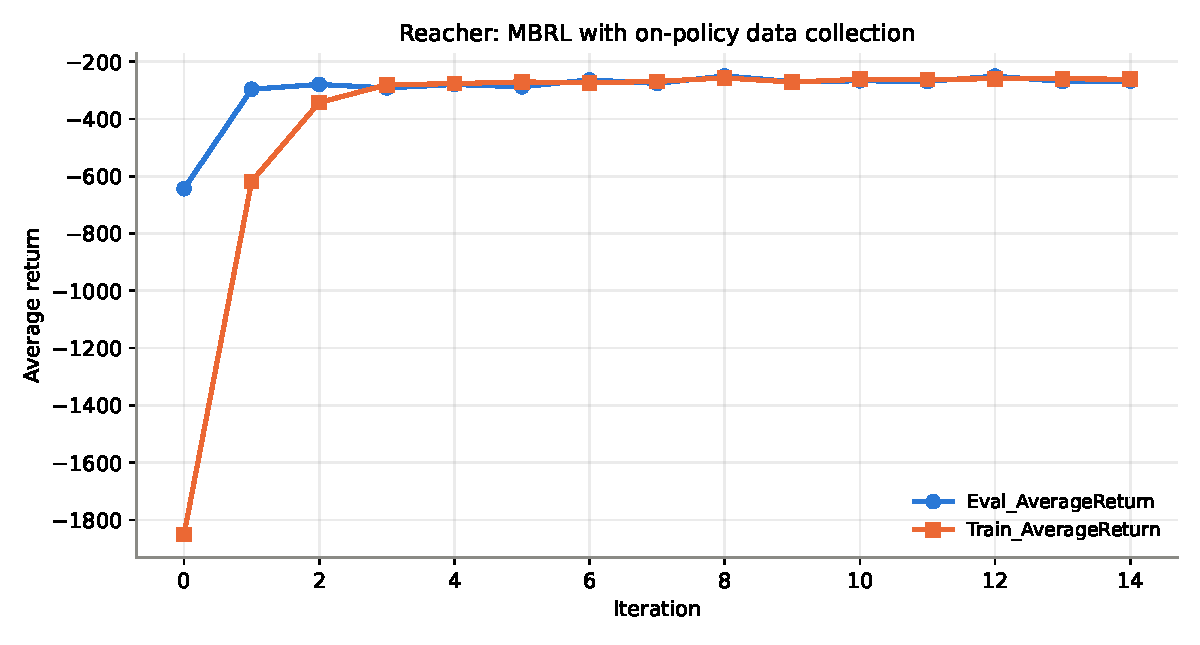
\includegraphics[width=\linewidth,height=8cm,keepaspectratio]{figures/q3_reacher.pdf}
\end{tcolorbox}
\begin{tcolorbox}[colback=white,colframe=black!60,title={Cheetah learning curve},height=9.5cm]
\centering
% Replace example-image-a with the path to your plot.
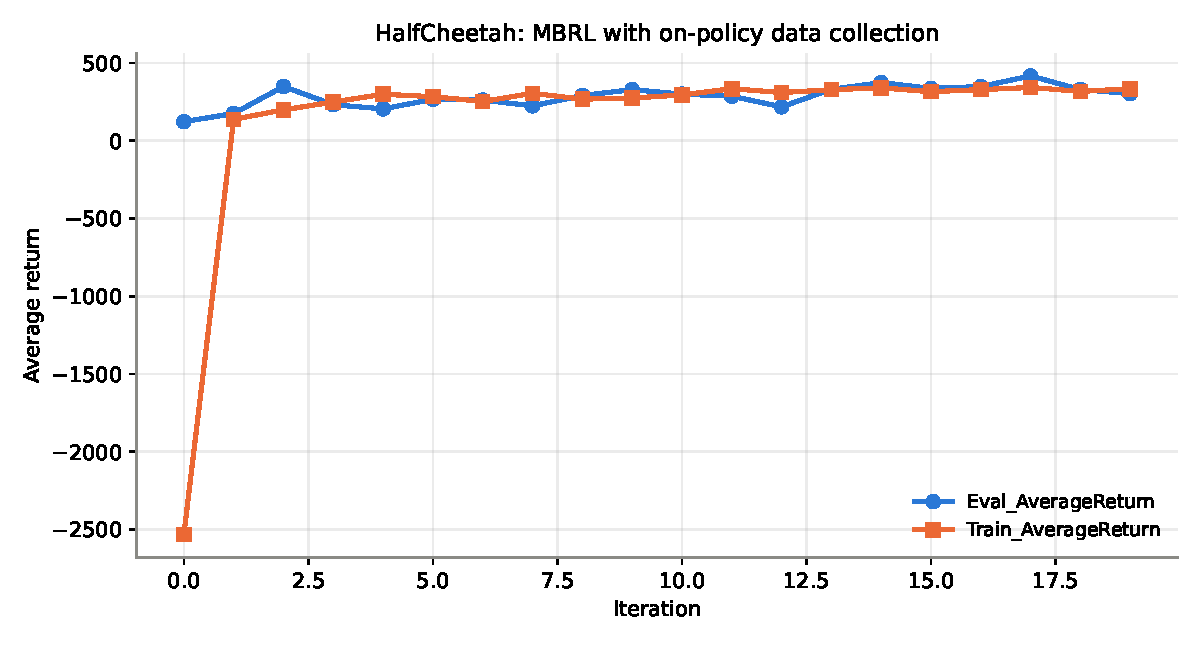
\includegraphics[width=\linewidth,height=8cm,keepaspectratio]{figures/q3_cheetah.pdf}
\end{tcolorbox}
\clearpage
\section*{Problem 4: Hyperparameter Comparison and Discussion (3.75 points total)}
\subsection*{Hyperparameter Comparison (3 points)}
For each comparison, describe the observed trend and explain it in the description block directly below the plot.
\begin{tcolorbox}[colback=white,colframe=black!60,title={Planning horizon: 5, 15, 30},height=9.5cm]
\centering
% Replace example-image-a with the path to your plot.
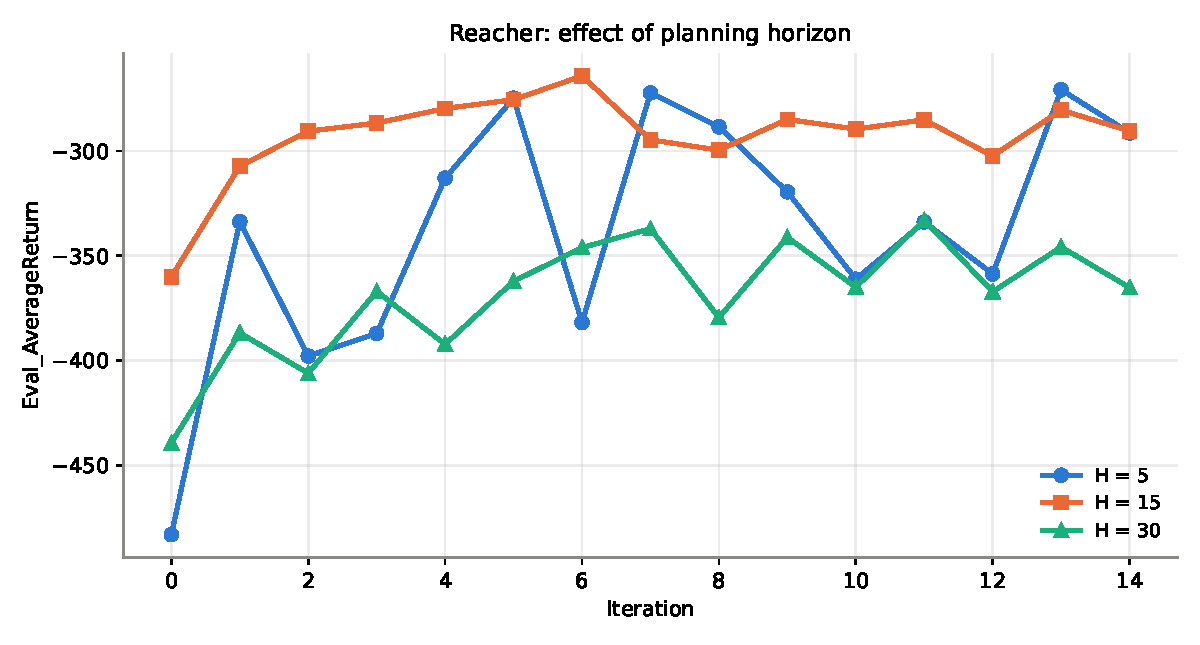
\includegraphics[width=\linewidth,height=8cm,keepaspectratio]{figures/q4_reacher_horizon.pdf}
\end{tcolorbox}
\begin{answer}{Description: planning horizon}
H = 15 gives the best and most stable return, with a mean of $-290$ over the last 5 iterations. H = 5 gives a mean of $-323$, and its return changes much between iterations. H = 30 gives the lowest return, with a mean of $-355$. For H = 5, a possible cause is that a short horizon cannot see the later effect of an action. For H = 30, a possible cause is that model error increases at each step, and random shooting finds fewer good sequences. These runs do not measure these causes directly.
\end{answer}
\newpage
\begin{tcolorbox}[colback=white,colframe=black!60,title={Candidate sequences: 100, 1000},height=9.5cm]
\centering
% Replace example-image-a with the path to your plot.
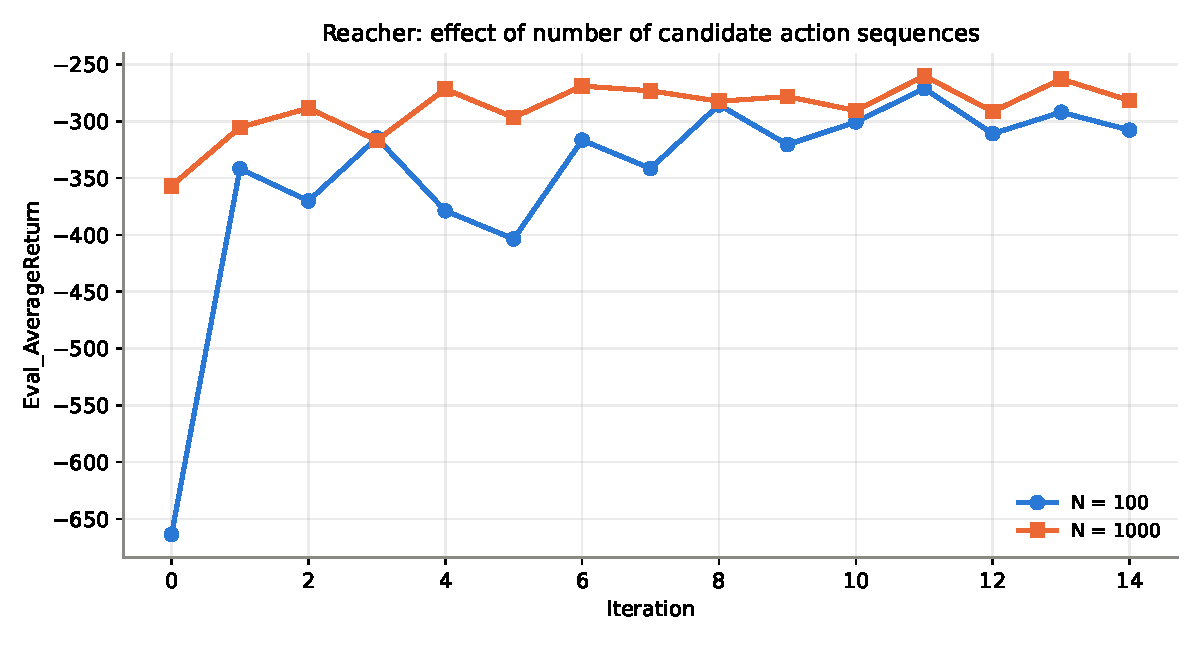
\includegraphics[width=\linewidth,height=8cm,keepaspectratio]{figures/q4_reacher_numseq.pdf}
\end{tcolorbox}
\begin{answer}{Description: number of candidate sequences}
N = 1000 gives a higher return than N = 100 at almost all iterations. The mean return over the last 5 iterations is $-277$ for N = 1000 and $-296$ for N = 100. N = 1000 is near its final return after 1 iteration, but N = 100 needs approximately 8 iterations. More candidate sequences cover the action space better, so the best sample can be nearer to the true optimum. The cost is time: the N = 1000 run takes approximately 4 times longer than the N = 100 run.
\end{answer}
\newpage
\begin{tcolorbox}[colback=white,colframe=black!60,title={Ensemble size: 1, 3, 5},height=9.5cm]
\centering
% Replace example-image-a with the path to your plot.
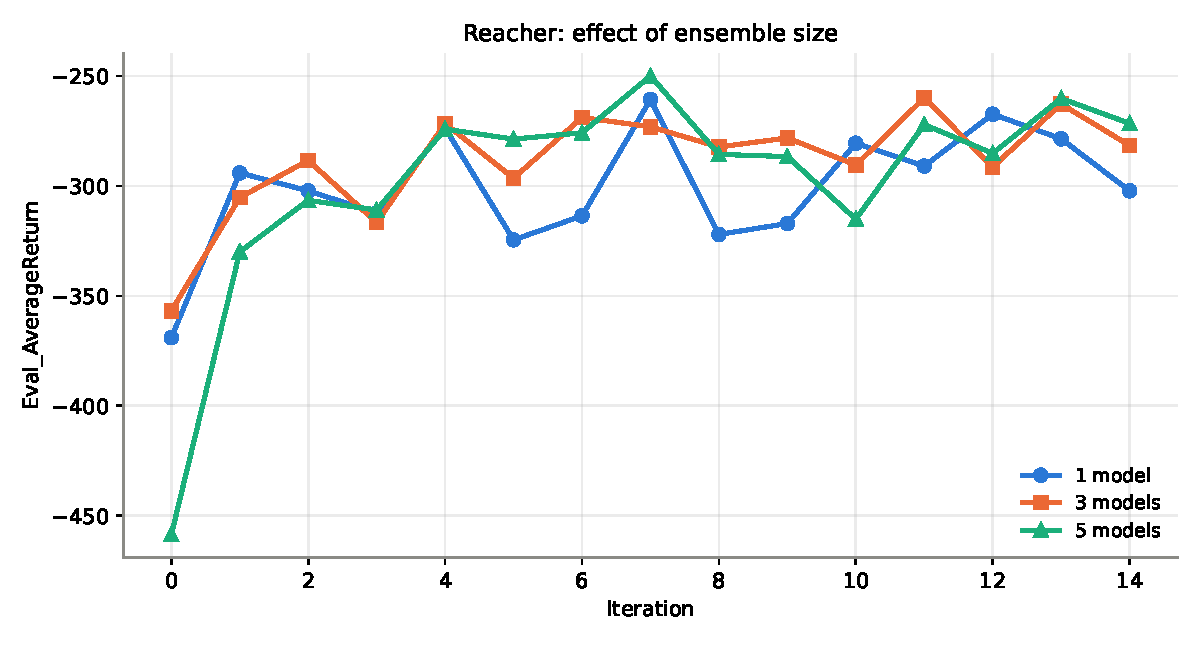
\includegraphics[width=\linewidth,height=8cm,keepaspectratio]{figures/q4_reacher_ensemble.pdf}
\end{tcolorbox}
\begin{answer}{Description: ensemble size}
The effect of ensemble size is small. The mean return over the last 5 iterations is $-284$ for 1 model, $-277$ for 3 models and $-281$ for 5 models. The single model has larger drops, for example at iterations 5, 8 and 9. A possible cause is that an ensemble averages the errors of independent models, so the planner finds fewer false high-reward sequences. 5 models take more time than 3 models, but give no clear gain. These results use only 1 seed, thus it is not possible to know if these small differences are reliable.
\end{answer}
\newpage
\subsection*{Discussion (0.75 points)}
Imagine you have a learned dynamics model that achieves low multi-step prediction error over the MPC planning horizon on held-out trajectories, but MPC using this model performs poorly. Give reasons why this could happen. Answer in 4--6 sentences.
\begin{answer}{Discussion answer}
Low error on held-out trajectories does not show low error on the states and actions that MPC selects. The planner selects the action sequence with the highest predicted reward, thus it finds the regions where the model predicts too high a reward. Random action sequences are often different from the actions in the held-out data, so the model can be wrong on them. Also, a small state error can cause a large reward error when the reward is sensitive to that state, for example near an obstacle. The MSE metric gives equal weight to all state dimensions, but the reward can depend on a few dimensions that the model predicts badly. Finally, a short horizon or too few candidate sequences can give bad actions, even with a perfect model.
\end{answer}
\end{document}
